\section{Giới thiệu}
\label{sec:gioi-thieu}

\subsection{Bối cảnh và động lực thực hiện}
\label{subsec:boi-canh}

Trong thập kỷ qua, sự thành công của các mô hình học sâu trong việc giải quyết những bài toán phức tạp của trí tuệ nhân tạo là điều không thể phủ nhận. Tuy nhiên, sự phát triển này lại đi kèm với những thách thức to lớn về mặt lý thuyết và thực tiễn, đặt ra yêu cầu cấp thiết về một khung toán học thống nhất và sự hiểu biết sâu sắc hơn về bản chất của các mô hình nơ-ron nhân tạo.

\subsubsection{Vấn đề phân mảnh kiến trúc và lời nguyền đa chiều}
\label{subsubsec:phan-manh-kien-truc}

Hạn chế đầu tiên và rõ rệt nhất của lĩnh vực học sâu hiện đại là sự thiếu vắng các nguyên lý thống nhất. Hiện nay, cộng đồng nghiên cứu đang chứng kiến sự bùng nổ của vô số kiến trúc mạng nơ-ron khác nhau, được thiết kế riêng biệt cho từng định dạng dữ liệu. Sự phân mảnh này dẫn đến tình trạng các khái niệm cơ bản liên tục được phát minh lại và định danh dưới những tên gọi khác nhau trong các lĩnh vực ứng dụng riêng biệt, làm lu mờ đi bản chất toán học cốt lõi của bài toán.

Bên cạnh đó, dưới góc độ lý thuyết học thống kê, việc xấp xỉ một hàm số tổng quát trong không gian đa chiều mà không dựa trên bất kỳ giả định tiên nghiệm nào là một bài toán bị chi phối nặng nề bởi lời nguyền đa chiều. Nếu chỉ dựa trên giả định về tính trơn cục bộ, độ phức tạp mẫu yêu cầu để học chính xác hàm mục tiêu sẽ tăng theo cấp số nhân so với số chiều của dữ liệu, khiến bài toán trở nên bất khả thi trong thực tế ngay cả với năng lực tính toán hiện đại.

\begin{infobox}{Khai thác tiên nghiệm hình học phá vỡ lời nguyền đa chiều}
Tuy nhiên, dữ liệu trong thế giới thực hiếm khi tồn tại dưới dạng các vector vô hướng ngẫu nhiên; chúng luôn mang theo những quy luật vật lý và cấu trúc hình học đặc thù, chẳng hạn như tính chu kỳ trong tín hiệu, cấu trúc lưới trong hình ảnh, hoặc các liên kết tô-pô trong phân tử hóa học. Việc khai thác các tiên nghiệm hình học này, đặc biệt là tính bất biến và tính đẳng biến thông qua lăng kính của \textit{Geometric Deep Learning}, đóng vai trò như một cơ chế lọc tự nhiên, giúp giới hạn triệt để không gian hàm cần tìm kiếm, qua đó trực tiếp phá vỡ lời nguyền đa chiều và cung cấp một bản thiết kế chung để hệ thống hóa toàn bộ các kiến trúc mạng hiện hành như CNN, RNN và GNN.
\end{infobox}

\subsubsection{Tính đối xứng tham số và học không gian trọng số}
\label{subsubsec:doi-xung-tham-so}

Trong các mô hình ngôn ngữ và mô hình sinh dữ liệu hiện nay, có một đặc điểm quan trọng: chúng thường có rất nhiều tham số (trọng số) hơn mức cần thiết. Vì vậy, tồn tại vô số cách sắp xếp trọng số khác nhau nhưng cuối cùng lại cho ra cùng một kết quả ở đầu ra.

Điều này xuất phát từ tính đối xứng trong không gian tham số. Khác với đối xứng dữ liệu đầu vào (như trong \textit{Geometric Deep Learning}), ở đây ta nói đến những phép biến đổi trực tiếp trên ma trận trọng số mà vẫn giữ nguyên hành vi của mạng. Nói cách khác, bạn có thể thay đổi trọng số theo nhiều cách khác nhau, nhưng mô hình vẫn hoạt động giống hệt. Sự tồn tại của những đa tạp chứa nhiều điểm cực tiểu tương đương này đã định hình cấu trúc của tổng quan của hàm mất mát. Nó tạo ra hiện tượng các cực tiểu được nối liền với nhau và khiến quá trình tối ưu hóa trở nên phức tạp hơn.

\begin{morong}[Xu hướng học không gian trọng số trong kỷ nguyên mô hình nền tảng]
Với sự bùng nổ của hàng triệu mô hình được lưu trữ trên các nền tảng mã nguồn mở, cộng đồng đang chứng kiến một hệ quả tất yếu là sự ra đời của hướng nghiên cứu học không gian trọng số. Hướng đi này coi chính các kiến trúc mạng nơ-ron là dữ liệu đầu vào, sử dụng \textit{meta-networks} để phân tích, nén và tinh chỉnh trực tiếp trên cấu trúc tham số. Trong kỷ nguyên của mô hình nền tảng, việc hiểu và tận dụng các đối xứng tham số linh hoạt thay vì \textit{hard-coding} trở thành chìa khóa để cải thiện định luật tỷ lệ và tăng cường hiệu quả tính toán.
\end{morong}


\subsubsection{Ý nghĩa và tầm quan trọng thực tiễn}
\label{subsubsec:y-nghia-thuc-tien}

Sự kết hợp giữa lý thuyết hình học của dữ liệu và tính đối xứng trong không gian tham số mang lại những bước tiến mang tính bản lề cho toàn bộ vòng đời của hệ thống học máy. Về mặt lý thuyết toán học, các chứng minh mới nhất cho thấy việc mã hóa tính đối xứng giúp cải thiện mạnh mẽ độ phức tạp mẫu, giảm thiểu nhu cầu dữ liệu lên đến nhiều bậc độ lớn, và gia tăng khả năng tổng quát hóa ngoài phân phối một cách nghiêm ngặt.

\begin{importantbox}{Ứng dụng khoa học mũi nhọn trong thế giới thực}
Hơn thế nữa, các mô hình học sâu dựa trên nền tảng hình học và đối xứng đang đóng vai trò trung tâm trong việc giải quyết những bài toán khoa học mũi nhọn. Từ việc mô phỏng hệ nguyên tử, dự đoán năng lượng tương tác phân tử, đến việc ứng dụng tính đẳng biến nhóm $SE(3)$ trong Robotics để điều khiển thao tác trong không gian vật lý, \textit{Geometric Deep Learning} đang chứng minh tiềm năng to lớn trong việc định hình các hệ thống trí tuệ nhân tạo có khả năng tương tác trực tiếp với các định luật vật lý của thế giới thực.
\end{importantbox}

\subsection{Kỷ nguyên của dữ liệu hình học}
\label{subsec:ky-nguyen-du-lieu-hinh-hoc}

Lĩnh vực học máy đang chứng kiến nỗ lực to lớn nhằm hợp nhất các mô hình phân mảnh thành một hệ thống lý thuyết chặt chẽ. Đóng góp nền tảng mang tính bước ngoặt cho nỗ lực này là công trình nghiên cứu \textit{Geometric Deep Learning: Grids, Groups, Graphs, Geodesics, and Gauges} của Bronstein và cộng sự (2021) \cite{bronstein2021geometric}. Hệ thống lý thuyết này được truyền cảm hứng sâu sắc từ chương trình Erlangen của nhà toán học Felix Klein, trong đó đề xuất rằng hình học nên được nghiên cứu thông qua các thuộc tính được bảo toàn dưới tác động của các nhóm phép biến đổi.

Nghiên cứu của Bronstein và cộng sự đã định hình lại cách các hệ thống trí tuệ nhân tạo tiếp nhận dữ liệu. Thay vì xử lý dữ liệu như các vector vô hướng, phương pháp này mô hình hóa dữ liệu dưới dạng các tín hiệu nằm trên năm miền hình học cơ bản, được hệ thống hóa thành khung 5G bao gồm Grids, Groups, Graphs, Geodesics và Gauges. Việc gắn kết dữ liệu vào các miền hình học cụ thể cho phép khai thác triệt để các quy luật tự nhiên, chẳng hạn như tính chu kỳ của ảnh trên miền Grids hay liên kết hóa học trên miền Graphs.

\begin{center}
    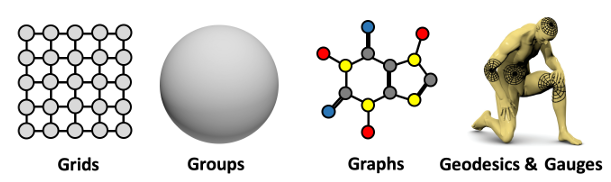
\includegraphics[width=0.85\textwidth, keepaspectratio]{graphics/5g_framework.png}
    
    \vspace{0.2cm}
    \captionof{figure}{Phân loại các miền hình học theo khung 5G}
    \label{fig:5g-framework}
\end{center}
\noindent\textit{Ghi chú: Các miền hình học cơ bản bao gồm Grids, Groups, Graphs, Geodesics và Gauges. Nguồn: \textit{Geometric Deep Learning: Grids, Groups, Graphs, Geodesics, and Gauges} (Bronstein et al., 2021).}

Từ sự phân loại này, một bản thiết kế chung được đề xuất nhằm chuẩn hóa cấu trúc của mạng nơ-ron. Cấu trúc này bao gồm bốn thành phần tính toán cốt lõi: lớp đồng biến tuyến tính, hàm kích hoạt phi tuyến, lớp gộp cục bộ để trích xuất đặc trưng đa tỷ lệ, và lớp gộp bất biến toàn cục ở cuối mạng. Trong đó, hai khái niệm toán học đóng vai trò nền tảng là Invariance và Equivariance. Invariance đảm bảo đầu ra của mô hình không thay đổi khi dữ liệu đầu vào bị biến đổi, trong khi Equivariance yêu cầu đầu ra phải biến thiên một cách tương ứng theo đúng phép biến đổi của đầu vào.

\begin{center}
    \begin{tikzpicture}[node distance=3.5cm, auto, thick, >=Stealth]
        \node (X) at (0, 0) {$\mathcal{X}$};
        \node (Y) at (3, 0) {$\mathcal{Y}$};
        \node (TX) at (0, -2.5) {$\mathcal{X}$};
        \node (TY) at (3, -2.5) {$\mathcal{Y}$};
        \draw[->] (X) -- node {$f$} (Y);
        \draw[->] (X) -- node[swap] {$\mathfrak{g}$} (TX);
        \draw[->] (Y) -- node {$\mathfrak{g}'$} (TY);
        \draw[->] (TX) -- node[swap] {$f$} (TY);
        \node[below=0.5cm of TX, xshift=1.5cm] {\textbf{(a) Equivariance}};
        \node (X2) at (6, 0) {$\mathcal{X}$};
        \node (Y2) at (9, -1.25) {$\mathcal{Y}$};
        \node (TX2) at (6, -2.5) {$\mathcal{X}$};
        \draw[->] (X2) -- node {$f$} (Y2);
        \draw[->] (X2) -- node[swap] {$\mathfrak{g}$} (TX2);
        \draw[->] (TX2) -- node[swap] {$f$} (Y2);

        \node[below=0.5cm of TX2, xshift=1.5cm] {\textbf{(b) Invariance}};
    \end{tikzpicture}
    
    \vspace{0.2cm}
    \captionof{figure}{Sơ đồ giao hoán toán học}
    \label{fig:commutative-diagram}
\end{center}
\noindent\textit{Ghi chú: (a) Tính đẳng biến (Equivariance): Biến đổi đầu vào tương đương với việc áp dụng phép biến đổi tương ứng lên đầu ra. (b) Tính bất biến (Invariance): Đầu ra không bị ảnh hưởng bởi phép biến đổi nhóm $\mathfrak{g}$.}

Bản thiết kế này cung cấp một khuôn khổ toán học minh bạch, chứng minh rằng các kiến trúc thành công nhất hiện nay như CNN, RNN, GNN và Transformer thực chất chỉ là các biến thể khác nhau của cùng một nguyên lý đối xứng khi áp dụng lên các miền dữ liệu hình học khác nhau.

\subsection{Sự dịch chuyển sang không gian trọng số}
\label{subsec:su-dich-chuyen-khong-gian-trong-so}

Nếu như giai đoạn đầu của Geometric Deep Learning tập trung giải quyết các bài toán liên quan đến đối xứng trong không gian dữ liệu, thì xu hướng nghiên cứu hiện đại đang chứng kiến một bước chuyển dịch chiến lược. Sự dịch chuyển này được khảo sát và hệ thống hóa một cách toàn diện trong nghiên cứu \textit{Symmetry in Neural Network Parameter Spaces} do Zhao và cộng sự (2026) thực hiện \cite{zhao2026symmetry}. Nhóm tác giả đã chuyển hướng phân tích trọng tâm từ dữ liệu đầu vào sang việc khám phá tính đối xứng nằm ngay bên trong cấu trúc tham số của mạng nơ-ron.

Theo phân tích của Zhao và cộng sự, các mô hình học sâu hiện đại thường ở trạng thái siêu tham số hóa, dẫn đến hiện tượng vô số cấu hình trọng số khác nhau nhưng lại sản sinh ra cùng một hàm tính toán ở đầu ra. Sự dư thừa này bắt nguồn từ các phép biến đổi nội tại, chẳng hạn như hoán vị các nơ-ron ẩn hoặc thay đổi tỷ lệ trọng số của hàm kích hoạt ReLU, mà không làm thay đổi giá trị dự đoán cuối cùng. Việc nhận diện Parameter space symmetry giúp giải mã cấu trúc phức tạp của Loss landscape, giải thích nguyên nhân hình thành các vùng bình nguyên và hiện tượng Mode connectivity giữa các điểm cực tiểu cục bộ.

\begin{morong}[Kỹ thuật Teleportation và Equivariant Metanetworks]
Khám phá này mở ra những kỹ thuật tối ưu hóa đột phá, điển hình là phương pháp Teleportation, cho phép thuật toán Gradient Descent chủ động dịch chuyển tham số đến các cấu hình tương đương mang đặc tính hội tụ tốt hơn. Quan trọng hơn, sự hiểu biết về đối xứng tham số là tiền đề cho lĩnh vực Weight space learning. Trong mô hình này, các tập hợp trọng số được xem như dữ liệu đầu vào cho một hệ thống Equivariant Metanetworks. Kiến trúc cấp cao này có khả năng dự đoán khả năng tổng quát hóa, nén mô hình và hợp nhất các điểm cực tiểu một cách hiệu quả mà không cần tiến hành suy luận trực tiếp trên dữ liệu gốc.
\end{morong}

\subsection{Mục tiêu và phạm vi của đồ án}
\label{subsec:muc-tieu-va-pham-vi}

\subsubsection{Mục tiêu nghiên cứu}
\label{subsubsec:muc-tieu-nghien-cuu}

Đồ án này hướng tới việc hệ thống hóa và thực nghiệm các kỹ thuật tiên tiến nhất trong lĩnh vực học máy hình học, dựa trên nền tảng lý thuyết từ các hội nghị đầu ngành. Việc tích hợp các tiên nghiệm hình học vào mô hình nhằm chứng minh ba lợi ích cốt lõi sau:

\begin{itemize}
    \item \textbf{Giảm bậc tự do và tăng Data efficiency:} Bằng cách ràng buộc không gian tìm kiếm thông qua các phép đối xứng, mô hình có thể đạt được độ chính xác cao với lượng dữ liệu huấn luyện ít hơn nhiều bậc độ lớn so với các phương pháp truyền thống.
    \item \textbf{Cải thiện OOD generalization và Robustness:} Kiến trúc tôn trọng các phép biến đổi hình học giúp hệ thống duy trì tính ổn định và khả năng ngoại suy chính xác khi đối mặt với dữ liệu nằm ngoài phân phối huấn luyện ban đầu.
    \item \textbf{Hỗ trợ các tác vụ tạo sinh:} Hiểu rõ cơ chế duy trì và phá vỡ đối xứng cung cấp nền tảng toán học vững chắc cho việc thiết kế các mô hình tạo sinh cấu trúc phức tạp như phân tử thuốc hay protein.
\end{itemize}

\subsubsection{Phạm vi và cấu trúc báo cáo}
\label{subsubsec:pham-vi-cau-truc}

Báo cáo tổng hợp các kỹ thuật từ nền tảng toán học cơ bản đến những hướng tiếp cận mới nhất về đối xứng tham số và học không gian trọng số. Nội dung chi tiết được cấu trúc thành sáu chương tiếp theo:

\begin{itemize}
    \item \textbf{Chương 2 (Kiến thức nền tảng):} Thiết lập cơ sở toán học cho báo cáo bằng cách giới thiệu lý thuyết nhóm, tác động nhóm, biểu diễn nhóm và khái niệm quỹ đạo. Chương này cũng trình bày các định nghĩa hình thức của tính bất biến và tính đẳng biến, làm tiền đề lý thuyết để xây dựng các mô hình nhận thức được hình học của dữ liệu.
    \item \textbf{Chương 3 (Các phương pháp xây dựng mô hình bảo toàn tính đối xứng):} Hệ thống hóa hai hướng tiếp cận chính để tích hợp tính đối xứng. Hướng thứ nhất can thiệp trên dữ liệu thông qua tăng cường dữ liệu, chuẩn hóa dữ liệu cùng định lý giới hạn về tính liên tục, lấy trung bình nhóm và lấy trung bình khung. Hướng thứ hai thiết kế kiến trúc tương biến từ đầu thông qua các lớp tuyến tính tương biến và cơ chế chia sẻ tham số như tích chập nhóm và DeepSets.
    \item \textbf{Chương 4 (Lý thuyết nâng cao và các hướng nghiên cứu mới):} Khảo sát các kết quả lý thuyết mới về độ phức tạp mẫu minimax optimal và các phương pháp tối ưu chi phí tính toán bằng đồ thị expander. Chương này cũng phân tích các bài toán kiểm định đối xứng trong dữ liệu, tính đối xứng không gian tham số của mạng nơ-ron, học không gian trọng số và các hướng mở rộng như mô hình không phụ thuộc số chiều hay học sâu tô-pô.
    \item \textbf{Chương 5 (Thực nghiệm và kết quả):} Trình bày các kết quả thực nghiệm định lượng trên các tập dữ liệu chuẩn để kiểm chứng lý thuyết. Các thực nghiệm bao gồm phân tích định luật tỷ lệ của NequIP trên QM9, kiểm chứng độ chính xác xấp xỉ lấy trung bình nhóm, học không gian trọng số qua mạng meta trên LoRA, gộp mô hình bằng căn chỉnh hoán vị Git Re-Basin và đánh giá định hướng của dữ liệu QM9.
    \item \textbf{Chương 6 (Đánh giá và kết luận):} Thảo luận chi tiết về các điều kiện áp dụng mô hình tương biến trong thực tế, bao gồm việc so sánh hiệu quả dữ liệu với định luật tỷ lệ khi tăng quy mô tính toán, phân biệt đối xứng chính xác và đối xứng xấp xỉ, đồng thời tổng hợp các ưu nhược điểm cốt lõi và định hướng phát triển tương lai.
    \item \textbf{Chương 7 (Demo minh họa):} Trình bày quá trình hiện thực hóa ba demo tương tác trên giao diện web sử dụng Next.js và FastAPI. Các demo minh họa hành vi của ba phương pháp: nhận diện chữ số viết tay bất biến với phép xoay trên MNIST, phân loại đám mây điểm bất biến với phép hoán vị bằng PointNet trên ModelNet40, và dự đoán năng lượng phân tử bất biến với nhóm Euclidean $E(3)$ bằng NequIP.
\end{itemize}

\clearpage